\documentclass[a4paper]{article}

\usepackage[english]{babel}
\usepackage[utf8]{inputenc}
\usepackage{amsmath}
\usepackage{graphicx}
\usepackage[colorinlistoftodos]{todonotes}

\title{RENDEZVOUS}

\author{Abhishek Agarwal(2014MCS2114)
\\ Harinder Pal(2014MCS2123)}

\date{\today}

\begin{document}
\maketitle

\begin{abstract}
\centering A Strategy game using OpenGL.
\end{abstract}

\section{Objective}

The following describes the design of a strategy game we plan to implement. The game revolves around two teams located on diagonally opposite sides of a map aiming to destroy each other's temple. Each team will have two players protecting the team's temple. Stating the obvious the team first to destroy the enemy temple wins.

\section{Play Modes}

We plan to offer two play modes for the end user. One being the \textbf{Bot Mode}, and other being the \textbf{MultiPlayer Mode}. In the \textbf{Bot Mode}, there will be one player with three AI players. The \textbf{MultiPlayer Mode} will allow four players on different nodes to play together, two players on each team.

\section{Outline of the game}
\begin{figure}[htp]
\centering
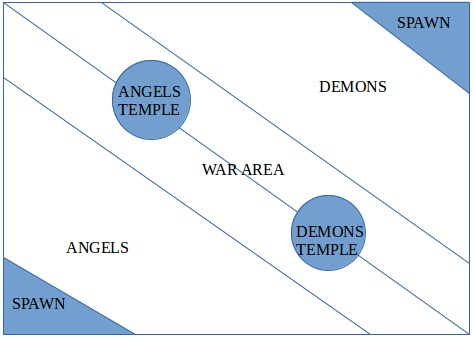
\includegraphics[width=0.7\textwidth]{outline.jpg}
\caption{\label{fig:outline}Bare outline of the map}
\end{figure}


\begin{enumerate}
\item Our game revolves around two teams Angels and Demons.

\item Each team will have its own team area on either side of the diagonal as shown in Figure. 1. The other team is not allowed to enter this area.

\item There is a common war area around the diagonal that both teams are allowed to enter.

\item The common war area around the diagonal will also have strategically located temples for each team.

\item There are 2 players per team. Therefore in total four players are allowed in MultiPlayer mode of the game.

\item The enemy team's team area is never visible.

\item The team's health is represented by the temple's health in the game. Destroying the enemy's temple means reducing enemy temple's health to zero.

\item Each player is assigned a hero. Each hero has his own health. Killing a hero means reducing it's health to zero. A hero is reborn after death in the team’s spawn area.

\item A team's temple health is considerably greater than it's individual hero's health.

\item The team area and war area will have obstacles(stones/trees) located. The hero will have to find paths around these obstacles to their target locations.

\item Each hero is allowed to move in horizontal and vertical direction. Once a target location is identified, the hero will use A* to reach the destination based on above restrictions.

\item The hero while traversing can pick certain items which add to its capabilities. The items are further described in the document.

\item Each hero will have a basic attacking capability and a magic power. Thus, each hero will have two modes of attack : Basic mode and Magic mode. Heros are further described in the document.

\item Each team will have it's own spawn area. A hero when born/re-born will find itself in this spawn area. Hero's can refuel their health by traversing back to this spawn area.
\end{enumerate}

\section{Schematic Map Representation}
We have internally divided our map area into a grid of 20 by 20. Consider the schematic diagram of our map in Figure 2. We have represented the map details for one team in a table. The other team area has been left blank for it is a copy and paste mirror image of the same around the diagonal.

\begin{figure}[htp]
\centering
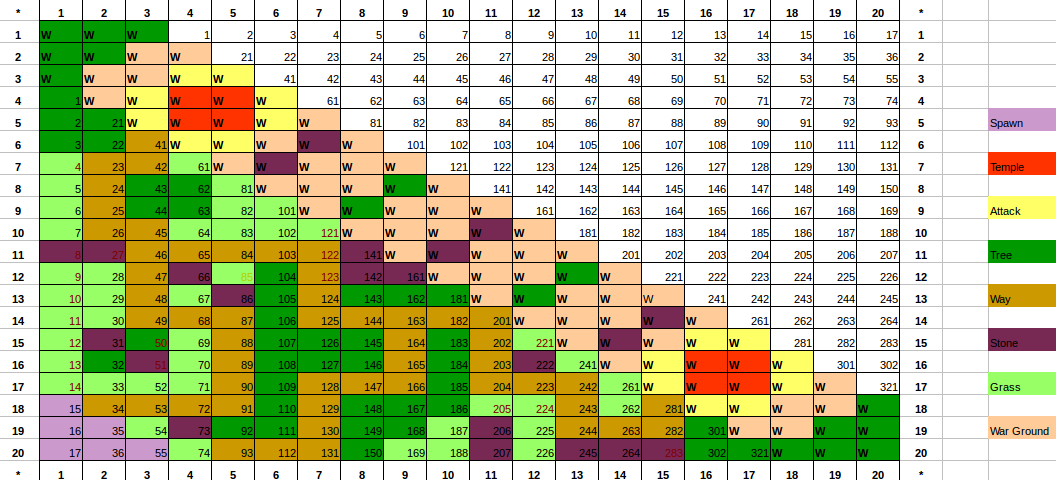
\includegraphics[width=1.1\textwidth]{Map_excel.png}
\caption{\label{fig:schematic}Schematic Map Representation}
\end{figure}


\section{Graphical Map Representation}
The graphical representation of our map respectively for both Demons and Angels is shown in Figure 3. Notice the visibility for both the teams. 

\begin{figure}[htp]
\centering
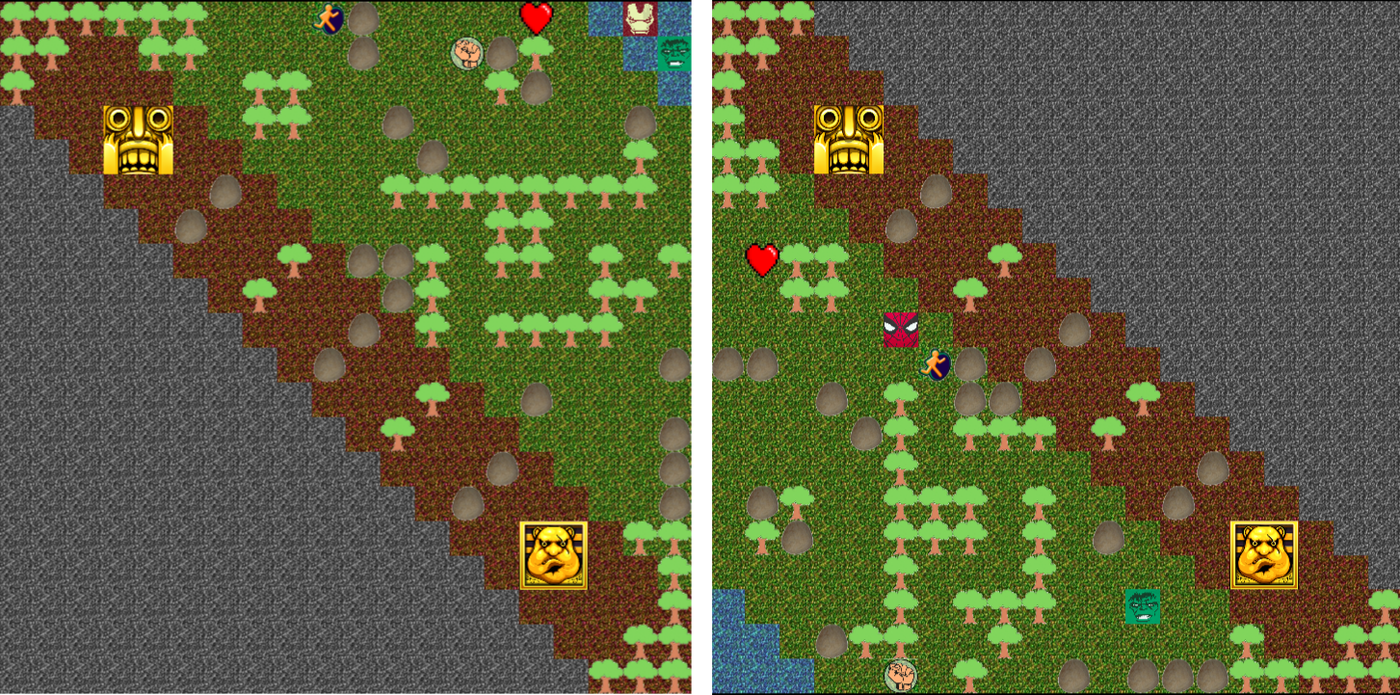
\includegraphics[width=1.0\textwidth]{Map_Views.png}
\caption{\label{fig:angels}Views of the Map}
\end{figure}


\section{Notification area}
The game is accompanied by an attribute area on both side of the maps, where the users can keep track of the game’s progress, etc. The schema for such an area is clearly depicted in Figure 4. 

\begin{figure}[htp]
\centering
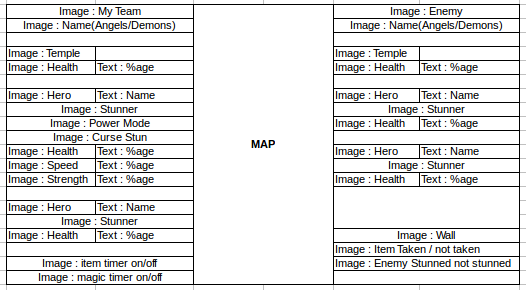
\includegraphics[width=0.9\textwidth]{attribute_space.png}
\caption{\label{fig:attribute}Schematic view of the attribute space}
\end{figure}


\section{Complete Map look}
The map in its entirety is shown in Figure 5. Notice the attribute area on either side.

\begin{figure}[htp]
\centering
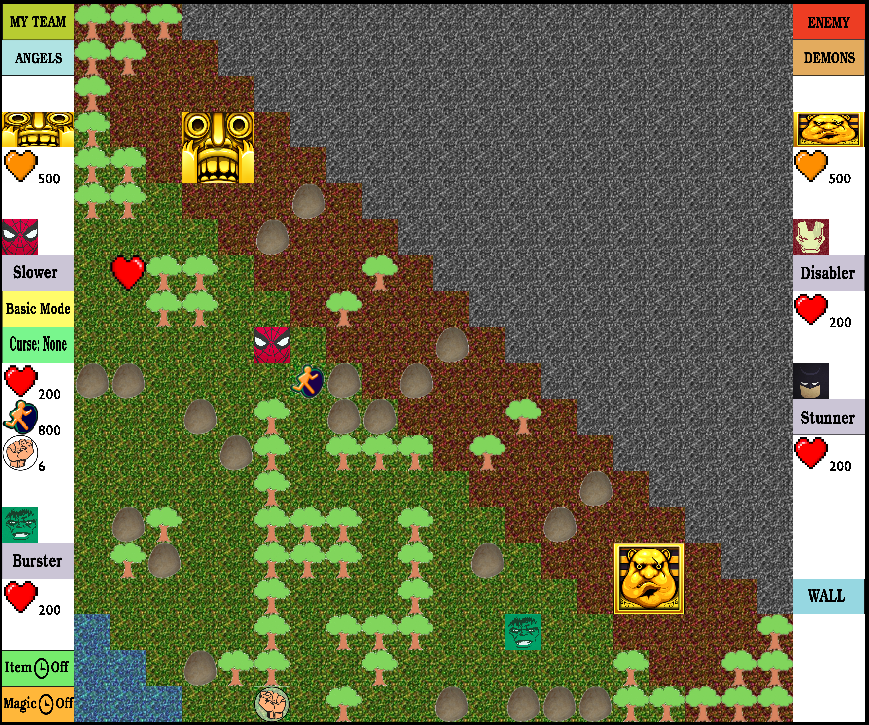
\includegraphics[width=0.7\textwidth]{Map_Attributes.png}
\caption{\label{fig:attributeMap}Complete Map with attribute space}
\end{figure}

\section{Hero Details}
We have four heroes to play with as shown in Figure 6.\\

\begin{figure}[htp]
\centering
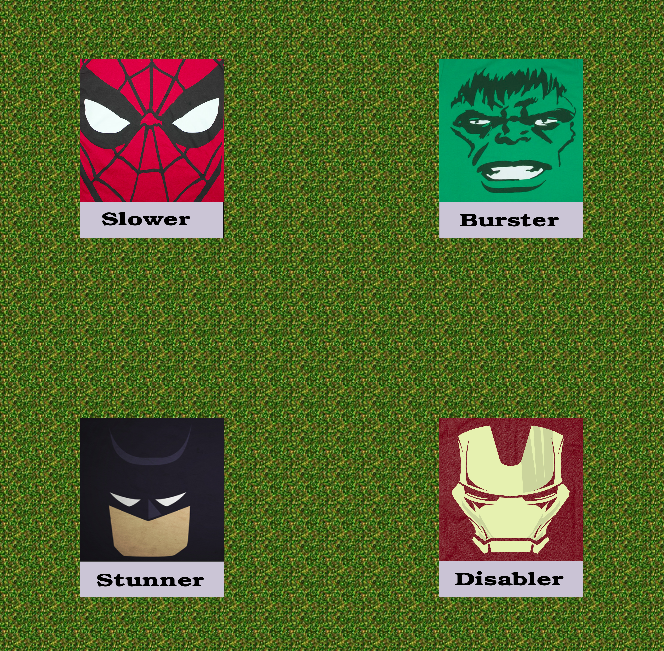
\includegraphics[width=0.5\textwidth]{Heros.png}
\caption{\label{fig:heroes}Heroes}
\end{figure}

Each hero has a unique magic power as described:
\begin{enumerate}
\item Stunner: Freezes the enemy player from attacking, moving, etc. for five seconds.
\item Slower: Slows down the enemy player for five seconds. Reduces its movement speed.
\item Disabler: Disables the enemy player from using any magical power for five seconds.
\item Burster: Does burst damage in a single shot.
\end{enumerate}

A hero is not allowed to use magic power in succession. It has to wait for some time before it can re-use the magic. \\

When a player uses it’s magic power on an enemy player, the enemy player is said to be cursed.

\section{Game Stats}
Each temple’s initial health is 500. Each hero’s initial heath is 200.
\\ \\
A hero has following attributes besides it’s health:
\begin{enumerate}
\item Strength: Damage done on a single attack (MIN 0 MAX 50)
\item Speed: Movement speed (MIN 100 MAX 1000)
\end{enumerate}

The above attributes depend on the hero type, as follows:
\begin{enumerate}
\item Stunner: Strength - 4, Speed - 600
\item Slower: Strength - 4, Speed - 700
\item Disabler: Strength - 6, Speed - 800
\item Burster: Strength - 6, Speed - 500
\end{enumerate}



\section{Item Details}
We have four items in our game. These items add to certain capabilities of the hero.
\begin{enumerate}
\item Speed Gain: Increases movement speed of the player by 25.
\item Strength Gain: Increases damage capability of the player by 1.
\item Temple Healer: Increases health of the player’s temple by 10.
\item Heath Gain: Increases health of the player by 5.
\end{enumerate}

\textit {The above stats are not final We will take into account fairness when deciding final stats as we proceed with the implementation.}

\end{document}